% Slides for ApacheCon US 2015
%
% Phil Steitz <phil.steitz@gmail.com>
% April 14, 2015

\documentclass[14pt,mathserif]{beamer}
\usetheme{Boadilla}

\setbeamertemplate{footline}
{
  \leavevmode%
  \hbox{%
    \begin{beamercolorbox}[wd=.333333\paperwidth,ht=2.25ex,dp=1ex,center]{author in head/foot}%
    \usebeamerfont{author in head/foot}\insertshortinstitute
    \end{beamercolorbox}%
    \begin{beamercolorbox}[wd=.333333\paperwidth,ht=2.25ex,dp=1ex,center]{title in head/foot}%
      \usebeamerfont{title in head/foot}\insertshorttitle
    \end{beamercolorbox}%
    \begin{beamercolorbox}[wd=.333333\paperwidth,ht=2.25ex,dp=1ex,right]{date in head/foot}%
      \usebeamerfont{date in head/foot}\insertshortdate{}\hspace*{2em}
      \insertframenumber{} / \inserttotalframenumber\hspace*{2ex}
    \end{beamercolorbox}}%
  \vskip0pt%
}

\usepackage[T1]{fontenc}
\usepackage{lmodern}
\usepackage{color}
\usepackage{minted}

%---- Copy the frame title color --------------------------%
\newcommand{\fblue}[1]{\usebeamercolor[fg]{frametitle}{#1}}

\newcommand{\newauthor}[2]{
  \parbox{0.26\textwidth}{
    \texorpdfstring
      {
        \centering
        #1 \\
        {\scriptsize{\urlstyle{same}\url{#2}\urlstyle{tt}}}
      }
      {#1}
  }
}

\hypersetup{colorlinks,linkcolor=cyan,urlcolor=blue}

%----------- Section title slides -----------------------------------%
\AtBeginSection[]{
  \begin{frame}
  \vfill
  \centering
  \begin{beamercolorbox}[sep=8pt,center,shadow=true,rounded=true]{title}
    \usebeamerfont{title}\secname\par%
  \end{beamercolorbox}
  \vfill
  \end{frame}
}

%gets rid of navigation symbols
\setbeamertemplate{navigation symbols}{}

\title{Programming Math in Java}
\subtitle{Lessons from Apache Commons Math}
\author{
  \newauthor{Phil Steitz}{psteitz@apache.org}
}
\institute[Apachecon North America 2015]{Apachecon North America 2015}
\date{April 14, 2015}
\begin{document}

%----------- titlepage ----------------------------------------------%
{
\begin{frame} %[plain]
  \titlepage
\end{frame}
}

%----------- slide --------------------------------------------------%
\begin{frame}
  \frametitle{Agenda}
\begin{itemize}
  \item Commons Math Overview
  \item Examples and problems
  \item Lessons learned
  \item Getting involved
\end{itemize}

\end{frame}

%----------- slide --------------------------------------------------%
\begin{frame}
  \frametitle{Disclaimer}

Apache Commons Math is a community-based, open development project. \\~\\
The discussion of problems, challenges and lessons learned represents one
contributor's views.

\end{frame}

%----------- slide --------------------------------------------------%
\begin{frame}
  \frametitle{Goals}

\begin{itemize}
  \item Self-contained, ASL-licensed Java
  \item Provide simple solutions to common problems
  \item Implement standard, well-documented algorithms
  \item Balance ease of use and good design
  \item Stay well-tested and maintained
  \item Maintain a strong community
\end{itemize}

\end{frame}

%----------- slide --------------------------------------------------%
\begin{frame}[fragile]
  \frametitle{}

\textbf{\fblue{Some Statistics}} (as of March 11, 2015)...

\begin{itemize}
\item 67 packages
\begin{itemize}
\item 908 classes
\item 84,057 lines of code
\end{itemize}
\item 54,629 lines of comments
\begin{itemize}
\item 99.7\% documented API
\end{itemize}
\item 5862 unit tests
\begin{itemize}
\item 92\% of code covered
\end{itemize}
\item 80 open issues
\begin{itemize}
\item Average 216 issues resolved per year
\end{itemize}
\item 6 active committers
\item 70+ contributors
\item 0 dependencies
\end{itemize}


\end{frame}


%----------- slide --------------------------------------------------%
\begin{frame}
  \frametitle{Message from our sponsors...}

\begin{columns}
\begin{column}{.5\textwidth}
\textbf{\fblue{Come join us!}}
\\
\setbeamertemplate{itemize items}[default]
\begin{itemize}
\item Code is interesting!
\item Math is interesting!
\item Bugs are interesting!
\item People are interesting!
\end{itemize}
\\
\textbf{\fblue{Come join us!}} \\
\end{column}
\begin{column}{.5\textwidth}\raggedleft

\includegraphics[width=6cm]{commons-logo.png}\\~\\

\includegraphics[width=5cm]{math.jpg}
\end{column}
\end{columns}
\\~\\
\url{http://commons.apache.org/math}
\end{frame}

%--------------------------------------------------------------------%
\section[Overview]{Quick Tour}

%----------- slide --------------------------------------------------%
\begin{frame}
  \frametitle{}

\textbf{\fblue{Building Blocks}} - util, special, complex packages

\begin{small}
\begin{itemize}
  \item FastMath (pure java replacement for java.lang.Math)
  \item Dfp (arbitrary precision arithmetic)
  \item Continued fractions
  \item Special functions (Beta, Gamma, Bessel, Erf)
  \item Array utilities (norms, normalization, filling, etc)
  \item Basic combinatorics (binomial coefficients, factorials, Stirling numbers..)
  \item Basic integer arithmetic (checked operations, gcd, lcm, primality...)
  \item Complex numbers
\end{itemize}
\end{small}
\end{frame}

%----------- slide --------------------------------------------------%
\begin{frame}
  \frametitle{}
  
\textbf{\fblue{Linear Algebra}} - linear package

\begin{small}
\begin{itemize}
  \item Vector and Matrix operations (dense, sparse, field)
  \item Decompositions (LU, QR, Cholesky, SVD, Eigenvalue)
  \item Solvers
\end{itemize}
\end{small}

\textbf{\fblue{Basic Numerical Analysis}} - analysis package

\begin{small}
\begin{itemize}
  \item Automatic Differentiation
  \item Numerical Integration
  \item Interpolation
  \item Root finders
\end{itemize}
\end{small}


\end{frame}

%----------- slide --------------------------------------------------%
\begin{frame}
  \frametitle{}

\textbf{\fblue{Probability and Statistics}} - distributions, stat and random packages

\begin{small}
\begin{itemize}
  \item Probability distributions
  \item Random number generators (Well, ISAAC, Mersenne twister...)
  \item Random data generators (samplers, random vectors, empirical density)
  \item Univariate statistics (storeless and in-memory)
  \item Regression (storeless bivariate, matrix-based and storeless multivariate)
  \item Correlation
  \item Inference (T-, G-, ChiSquare, Kolmogorov-Smirnov tests...)  
\end{itemize}
\end{small}
\end{frame}

%----------- slide --------------------------------------------------%
\begin{frame}
  \frametitle{}
  
\textbf{\fblue{Optimization and Geometry}} - optim, fitting, ode, transform,
geometry packages

 \begin{small}
 \begin{itemize}
  \item Fitting (non-linear least-squares, curve fitting)
  \item Ordinary differential equations (ODE)
  \item Linear/Non-linear optimization
  \item Computational Geometry
  \item Fast Fourier transform
 \end{itemize}
\end{small}
\end{frame}

%----------- slide --------------------------------------------------%
\begin{frame}
  \frametitle{}

\textbf{\fblue{AI / Machine learning}} - genetics, filter and ml packages

\begin{small}
\begin{itemize}
  \item Genetic algorithms
  \item Neural networks
  \item Clustering
  \item Kalman filter
\end{itemize}
\end{small}
\end{frame}

%--------------------------------------------------------------------%
\section[Examples]{Examples and Challenges}
%----------- slide --------------------------------------------------%
\begin{frame}[fragile]
  \frametitle{Example 1 - Root finding}

\begin{small}
Find all roots of the polynomial \[p(x) = x^5 + 4x^3 + x^2 + 4 = (x+1)(x^2-x+1)(x^2+4)\]
\end{small}
\begin{minted}[xleftmargin=10pt,fontsize=\footnotesize,linenos=false]{java}

double[] coefficients = { 4.0, 0.0, 1.0, 4.0, 0.0, 1.0 };
LaguerreSolver solver = new LaguerreSolver();
Complex[] result = solver.solveAllComplex(coefficients, 0);
\end{minted}
\end{frame}

%----------- slide --------------------------------------------------%
\begin{frame}[fragile]
  \frametitle{Example - Root finding (cont)}

How about this one? \[p(x) = \prod\limits_{i=1}^{50}{15,000(i + ix + ix^2 + ix^3)}\]
As of 3.4.1, this will appear to hang.\\
Two problems:
\begin{enumerate}
  \item Complex iterates "escape to NaN"
  \item Default max function evaluations is set to Integer.MAX\_VALUE
\end{enumerate}
\end{frame}

%----------- slide --------------------------------------------------%
\begin{frame}[fragile]
  \frametitle{Example 1 - Root finding (cont)}

\begin{small}  
 First problem:  escape to NaN
\begin{itemize}
  \item Long and painful history debating C99x Annex G
  \item Desire: clear, self-contained, open documentation
  \item Desire: simple, performant code
  \item Result: use standard definitions and let NaNs propagate
\end{itemize}
Second problem: hanging
\begin{itemize}
  \item Ongoing debate about what to make defaults, whether to have defaults at all...
  \item Ease of use vs foot-shooting potential
  \item OO vs procedural / struct / primitives design
\end{itemize}
\end{small}
\end{frame} 
%----------- slide --------------------------------------------------%
\begin{frame}[fragile]
  \frametitle{Example 2 - Kolmogorov-Smirnov Test}

\begin{small}
\textbf{Problem:}  Given two samples \(S_1\) and \(S_2\), are they drawn from the
same underlying probability distribution?
\end{small}
\\
\begin{minted}[xleftmargin=10pt,fontsize=\footnotesize,linenos=false]{java}

// load sample data into double[] arrays
double[] s1 = ... 
double[] s2 = ...
KolmogorovSmirnovTest test = new KolmogorovSmirnovTest();

// Compute p-value for test
double pValue = test.kolmogorovSmirnovTest(s1, s2);

\end{minted}
\end{frame}

%----------- slide --------------------------------------------------%
\begin{frame}
  \frametitle{K-S Test Implementation Challenges}
\begin{small}
Test statistic \( = D_{m,n} = \) maximum difference between the empirical
distribution functions of the two samples. \\
 \begin{itemize}
  \item The distribution of \(D_{m,n}\) is asymptotically an easy-to-compute distribution
  \item For very small m, n, the distribution can be computed exactly, but expensively
  \item What to do for mid-size samples (m, n between 100 and 10000)?
  \item Should this distribution be in the distributions package?
  \item Reference data / correctness very hard to verify
 \end{itemize}
\end{small}
\end{frame}
%----------- slide --------------------------------------------------%
\begin{frame}[fragile]
  \frametitle{Example 3 - Multivariate optimization}

\begin{small}
Find the minimum value of \(100(y-x^2)^2 + (1-x)^2\), starting at the point \((-1, 1)\)
\end{small}
\\
\begin{minted}[xleftmargin=10pt,fontsize=\scriptsize,linenos=false]{java}

MultivariateFunction f = new MultivariateFunction() {
    public double value(double[] x) {
        double xs = x[0] * x[0];
        return (100 * FastMath.pow((x[1] -  xs), 2)) +
           FastMath.pow(1 - x[0], 2);
    }
};
PowellOptimizer optim = new PowellOptimizer(1E-13, 1e-40);
PointValuePair result = optim.optimize(new MaxEval(1000),
                        new ObjectiveFunction(f),
                        GoalType.MINIMIZE,
                        new InitialGuess(new double[] {-1, 1}));
\end{minted}
\\
\begin{small}
Works OK in this case, but...
\end{small}
\end{frame}

%----------- slide --------------------------------------------------%
\begin{frame}[fragile]
  \frametitle{Example 3 - Optimization (cont)}

\begin{small}
\\
{\fblue User question:} How do I choose among the available optimizers? \\
{\fblue Developer question:} How do we define a consistent API? \\

Another solution for Example 3:

\begin{minted}[xleftmargin=8pt,fontsize=\scriptsize,linenos=false]{java}

BOBYQAOptimizer optim = new BOBYQAOptimizer(4);
PointValuePair result = optim.optimize(new MaxEval(1000),
                        new ObjectiveFunction(f),
                        GoalType.MINIMIZE,
                        new InitialGuess(new double[] {-1, 1}),
                        SimpleBounds.unbounded(2));
\end{minted}
\\
Note additional parameter to optimize.

\end{small}
\end{frame}

%----------- slide --------------------------------------------------%
\begin{frame}[fragile]
  \frametitle{Example 3 - Optimization (cont)}

\begin{small}
To allow arbitrary parameter lists, we settled on varargs...

\begin{minted}[xleftmargin=10pt,fontsize=\scriptsize,linenos=false]{java}
public abstract class BaseOptimizer<PAIR>
...
/**
 * Stores data and performs the optimization.
 * 
 * The list of parameters is open-ended so that sub-classes can extend it
 * with arguments specific to their concrete implementations.
 * 
 * When the method is called multiple times, instance data is overwritten
 * only when actually present in the list of arguments: when not specified,
 * data set in a previous call is retained (and thus is optional in
 * subsequent calls).
...
 * @param optData Optimization data.
...
 */
public PAIR optimize(OptimizationData... optData)
\end{minted} 
\end{small}
\end{frame}

%----------- slide --------------------------------------------------%
\begin{frame}[fragile]
  \frametitle{Example 3 - Optimization (cont)}

Some additional challenges:

\begin{small}
\begin{itemize}
\item Stochastic algorithms are tricky to test
\item FORTRAN ports create awful Java code, but "fixing" can create discrepancies
\item BOBYQAOptimizer port has never really been fully supported
\item Answering user questions requires expertise and time
\end{itemize} 
\end{small}
\end{frame}
%----------- slide --------------------------------------------------%
\begin{frame}[fragile]
  \frametitle{Example 4 - Aggregated statistics}

\begin{small}
\\
Problem: Aggregate summary statistics across multiple processes
\end{small}

\begin{minted}[xleftmargin=10pt,fontsize=\scriptsize,linenos=false]{java}
// Create a collection of stats collectors
Collection<SummaryStatistics> aggregate =
     new ArrayList<SummaryStatistics>();
     
// Add a collector, hand it out to some process
// and gather some data...
SummaryStatistics procStats = new SummaryStatistics();
aggregate.add(procStats);
procStats.addValue(wildValue);
...
// Aggregate results
StatisticalSummary aggregatedStats =
     AggregateSummaryStatistics.aggregate(aggregate);

\end{minted}

\begin{small}
\begin{itemize}
\item SummaryStatistics instances handle large data streams
\item StatisticalSummary is reporting interface
\end{itemize}
Question: how to distribute instances / workload?
\end{small}
\end{frame}

%----------- slide --------------------------------------------------%
\begin{frame}
  \frametitle{Threading and workload management}

\textbf{Questions:}

\begin{enumerate}
\item Should we implement multi-threaded algorithms?
\item How can we be more friendly for Hadoop / other distributed compute environments?
\end{enumerate}
\\
\setbeamertemplate{itemize items}[default]
\begin{itemize}
\item So far (as of 3.4.1), we have not done 1. 
\item So far, answer to 2 has been "leave it to users." 
\end{itemize}
\fblue{Could be both answers are wrong...}
\end{frame}

%----------- slide --------------------------------------------------%
\begin{frame}[fragile]
  \frametitle{Example 5 - Genetic algorithm}

\begin{small}
Another example where concurrent execution would be natural...
\end{small}
\begin{minted}[xleftmargin=10pt,fontsize=\scriptsize,linenos=false]{java}
// initialize a new genetic algorithm
GeneticAlgorithm ga = new GeneticAlgorithm(
            new OnePointCrossover<Integer>(),
            CROSSOVER_RATE, 
            new BinaryMutation(),
            MUTATION_RATE,
            new TournamentSelection(TOURNAMENT_ARITY)
);

// initial population 
Population initial = getPopulation(); 

// stopping conditions
StoppingCondition stopCond = new FixedGenerationCount(NUM_GENERATIONS);

// run the algorithm
Population finalPopulation = ga.evolve(initial, stopCond);

// best chromosome from the final population
Chromosome bestFinal = finalPopulation.getFittestChromosome();

\end{minted}
 
\begin{small}
Question: how to distribute "evolve" workload?
\end{small}
\end{frame}

%----------- slide --------------------------------------------------%
\begin{frame}[fragile]
  \frametitle{Example 6 - OLS regression}

\begin{small}
Three ways to do it
\begin{description}
  \item[OLSMultipleRegression (stat.regression)] in-memory
  \item[MillerUpdatingRegression (stat.regression)] streaming
  \item[LevenbergMarquardtOptimizer (fitting.leastsquares)] in-memory
\end{description}
\begin{enumerate}
\item How to make sure users discover the right solution for them?
\item How much dependency / reuse / common structure to force?
\end{enumerate}
\end{small}
\end{frame}


%----------- slide --------------------------------------------------%
\begin{frame}[fragile]
  \frametitle{Example 6 - OLS regression (cont)}

\begin{small}
Simplest, most common:
\begin{minted}[xleftmargin=10pt,fontsize=\scriptsize,linenos=false]{java}
OLSMultipleLinearRegression regression = new OLSMultipleLinearRegression();

// Load data
double[] y = new double[]{11.0, 12.0, 13.0, 14.0, 15.0, 16.0};
double[] x = new double[6][];
x[0] = new double[]{0, 0, 0, 0, 0};
x[1] = new double[]{2.0, 0, 0, 0, 0};
...
x[5] = new double[]{0, 0, 0, 0, 6.0};          
regression.newSample(y, x);

// Estimate model
double[] beta = regression.estimateRegressionParameters();       
double[] residuals = regression.estimateResiduals();
double rSquared = regression.calculateRSquared();
double sigma = regression.estimateRegressionStandardError();
\end{minted}
Question:  What happens if design matrix is singular?
\end{small}
\end{frame}

%----------- slide --------------------------------------------------%
\begin{frame}[fragile]
  \frametitle{Example 6 - OLS regression (cont)}

\begin{small}
\textbf{Answer:} if it is "exactly" singular, \mintinline{latex}{SingularMatrixException}
\\~\\
If it is near-singular, garbage out \\
So make singularity threshold configurable:
\begin{minted}[xleftmargin=10pt,fontsize=\scriptsize,linenos=false]{java}
OLSMultipleLinearRegression regression =
     new OLSMultipleLinearRegression(threshold);
\end{minted}
\setbeamertemplate{itemize items}[default]
\begin{itemize}
\item What exactly is this threshold?
\item What should exception error message say?
\item How to doc it?
\item What if we change underlying impl?
\end{itemize}
\end{small}
\end{frame}

%-------------- slide -----------------------------------------------%
\begin{frame}[fragile]
  \frametitle{Example 7 - Rank correlation}

Given two double arrays \mintinline{latex}{x[]} and \mintinline{latex}{y[]}, we want
a statistical measure of how well their rank orderings match. \\ ~ \\
Use Spearman's rank correlation coefficient.

\begin{minted}[xleftmargin=10pt,fontsize=\scriptsize,linenos=false]{java}
double[] x = ...
double[] y = ...
SpearmansCorrelation corr = new SpearmansCorrelation();
corr.correlation(x, y);
\end{minted}

How are ties in the data handled? \\
What if one of the arrays contains NaNs?
\end{frame}

%-------------- slide -----------------------------------------------%
\begin{frame}
  \frametitle{Example 7 - Rank correlation (cont)}

\begin{small}
\begin{itemize}
\item As of 3.4.1, by default ties are averaged and NaNs causes RTE
\item Both are configurable via RankingAlgorithm constructor argument
\item RankingAlgorithm is a ranking implementation plus
\begin{itemize}
  \item TiesStrategy - what ranks to assign to tied values
  \item NaNStrategy - what to do with NaN values
\end{itemize}
\item Default in Spearman's is natural ranking on doubles with ties averaged and NaNs disallowed
\end{itemize}
Problems: 
\begin{enumerate}
\item What if user supplies a NaturalRanking with the NaN strategy that says remove NaNs? 
\item How to doc clearly and completely?
\end{enumerate}
\end{small}
\end{frame}

%----------- slide --------------------------------------------------%
\begin{frame}[fragile]
  \frametitle{Example 8 - Random Numbers}
  
\begin{small} 
Commons Math provides alternatives to the JDK PRNG and a pluggable framework
\setbeamertemplate{itemize items}[default]
\begin{itemize}
\item RandomGenerator interface is like j.u.Random
\item All random data generation within Commons Math is pluggable
\end {itemize}
Well generator is usually the default \\
Low-level example:
\begin{minted}[xleftmargin=10pt,fontsize=\scriptsize,linenos=false]{java}
// Allocate an array to hold random bytes
byte[] bytes = new byte[20];

// Instantiate a Well generator with seed = 100;
Well19937c gen = new Well19937c(100);

// Fill the array with random bytes from the generator
gen.nextBytes(bytes);
\end{minted}
\end{small}
\end{frame}

%----------- slide --------------------------------------------------%
\begin{frame}[fragile]
  \frametitle{Example 8 - Random Numbers (cont)}  
  
High-level example:

\begin{minted}[xleftmargin=10pt,fontsize=\footnotesize,linenos=false]{java}
 // Create a RandomDataGenerator using a Mersenne Twister 
 RandomDataGenerator gen = 
      new RandomDataGenerator(new MersenneTwister());
      
 // Sample a random value from the Poisson(2) distribution
 long dev = gen.nextPoisson(2);
 \end{minted}

Problems:
\begin{small}
\begin{enumerate}
\item Well generators (used as defaults a lot) have some initialization overhead.
How / when to take this hit
\item Distribution classes also have sample() methods, but that makes them dependent on
generators
\end{enumerate}
\end{small}
\end{frame}

%----------- slide --------------------------------------------------%
\begin{frame}[fragile]
  \frametitle{Example 9 - Linear Programming} 

\begin{small}
Maximize \(7x_1 + 3x_2\) subject to \\
\(3x_1 - 5x_3 \leq 0\) \\
\(2x_1 -5x_4 \leq 0\) \\
... (more constraints)

\begin{minted}[xleftmargin=10pt,fontsize=\scriptsize,linenos=false]{java}
LinearObjectiveFunction f = 
  new LinearObjectiveFunction(new double[] { 7, 3, 0, 0 }, 0 );

List<LinearConstraint> constraints = new ArrayList<LinearConstraint>();
constraints.add( new LinearConstraint(new double[] { 3, 0, -5, 0 },
                                      Relationship.LEQ, 0.0));  
constraints.add(new LinearConstraint(new double[] { 2, 0, 0, -5 },
                                      Relationship.LEQ, 0.0));
...
SimplexSolver solver = new SimplexSolver();
PointValuePair solution = solver.optimize(new MaxIter(100), f,
                          new LinearConstraintSet(constraints),
                          GoalType.MAXIMIZE,
                          new NonNegativeConstraint(true));
\end{minted}
\end{small}
\end{frame}

%----------- slide --------------------------------------------------%
\begin{frame}[fragile]
  \frametitle{Example 9 - Linear Programming (cont)} 
\\ 
\begin{small}
\textbf{Question:} What happens if the algorithm does not converge? \\
\textbf{Answer:} \mintinline{latex}{TooManyIterationsException} \\~\\
What if I want to know the last \mintinline{latex}{PointValuePair}?

\begin{minted}[xleftmargin=10pt,fontsize=\scriptsize,linenos=false]{java}
SolutionCallback callback = new SolutionCallback();
try {
    PointValuePair solution = solver.optimize(new MaxIter(100), f,
                          new LinearConstraintSet(constraints),
                          GoalType.MAXIMIZE,
                          new NonNegativeConstraint(true), callback);
} catch (TooManyIterationsException ex) {
	PointValuePair lastIterate = callback.getSolution();
}
\end{minted}

(Rejected) Alternatives:
\begin{enumerate}
\item Don't throw, but embed some kind of status object in return
\item Shove context data in exception messages
\end{enumerate}
\end{small}
\end{frame}

%----------- slide --------------------------------------------------%
\begin{frame}[fragile]
  \frametitle{Example 10 - Geometry} 

\begin{small}
Calculate the convex hull and enclosing ball of a set of 2D points:

\begin{minted}[xleftmargin=10pt,fontsize=\scriptsize,linenos=false]{java}
List<Vector2D> points = ...
ConvexHullGenerator2D generator = new MonotoneChain(true, 1e-6);
ConvexHull2D hull = generator.generate(points);

Encloser<Euclidean2D, Vector2D> encloser =
  new WelzlEncloser<Euclidean2D, Vector2D>(1e-6, new DiskGenerator());
EnclosingBall<Euclidean2D, Vector2D> ball = encloser.enclose(points);
\end{minted}
\end{small}

\\
\begin{columns}
\begin{column}{.5\textwidth}
\begin{small}
Problems:
\begin{enumerate}
\item algorithms are prone to numerical problems
\item important to specify a meaningful tolerance, but depends on input data
\item does it make sense to support a default tolerance?
\end{enumerate}
\end{small}
\end{column}
\begin{column}{.5\textwidth}\raggedleft
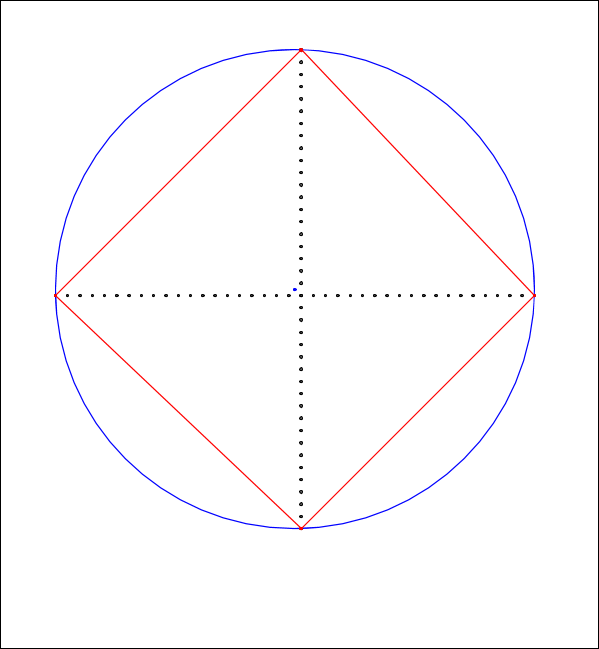
\includegraphics[width=4cm]{geometry.png}
\end{column}
\end{columns}

\end{frame}

%--------------------------------------------------------------------%
\section[Getting involved]{Lessons Learned}
%----------- slide --------------------------------------------------%
\begin{frame}
  \frametitle{Key Challenges Recap...}

\begin{small}
\begin{itemize}
\item Balancing performance, mathematical correctness and algorithm fidelity
\item Fully documenting behavior and API contracts
\item Steering users toward good solutions as simply as possible
\item Balancing OO design and internal reuse with approachability 
\item Obscure and abandoned contributions 
\item Reference implementations and / or data for validation
\item Backward compatibility vs API improvement
\end{itemize}
\end{small}
\end{frame}

%----------- slide --------------------------------------------------%
\begin{frame}
  \frametitle{Some lessons learned}

\begin{small}
\begin{itemize}
\item Let practical use cases drive performance / accuracy / fidelity decisions
\item Be careful with ports and large contributions
\item Limit public API to what users need
\item Prefer standard definitions and algorithms
\item Take time to fully research bugs and patches
\item Constantly improve javadoc and User Guide
\item Try to avoid compatibility breaks, but bundle into major
version releases when you have to
\end{itemize}
\end{small}
\end{frame}

%--------------------------------------------------------------------%
\section[Getting involved]{Get Involved!}
%----------- slide --------------------------------------------------%
\begin{frame}[fragile]
  \frametitle{Using Apache Commons Math}

Maven:

\begin{minted}[xleftmargin=10pt,fontsize=\small,linenos=false]{xml}

<dependency>
    <groupId>org.apache.commons</groupId>
    <artifactId>commons-math3</artifactId>
    <version>3.4.1</version>
</dependency>
\end{minted}

Download:\\
\begin{small}
\url{http://commons.apache.org/math/download_math.cgi} \\
\end{small}
\\
Watch for new versions!           
\end{frame}

%----------- slide --------------------------------------------------%
\begin{frame}
  \frametitle{Links}

\begin{small}
\begin{itemize}
  \item Project homepage: \url{http://commons.apache.org/math/}
  \item Issue tracker: \url{https://issues.apache.org/jira/browse/MATH}
  \item Mailinglists: dev@commons.apache.org \& user@commons.apache.org \\
  e-mail subject: [math]
  \item Wiki: \url{http://wiki.apache.org/commons/MathWishList}
\end{itemize}
\end{small}
\end{frame}

%----------- slide --------------------------------------------------%
\begin{frame}
  \frametitle{How to contribute?}

\begin{itemize}
  \item Check out the user guide \url{http://commons.apache.org/math/userguide/index.html}
  \item Ask questions on the user mailinglist
  \item Participate in discussions on the dev mailinglist
  \item Create bug reports / feature requests / improvements in JIRA
  \item Send patches (code, documentation, examples)
  \item Provide feedback - most welcome!
\end{itemize}

\end{frame}

%----------- slide --------------------------------------------------%
\begin{frame}
  \frametitle{}

\begin{itemize}
  \item Questions?
\end{itemize}

\end{frame}

\end{document}
